\documentclass[12pt]{article}
\usepackage[margin=2cm]{geometry}
\usepackage{amsmath}
\usepackage{graphicx}

\begin{document}

\noindent
The following table of hydrogen transition data is from
``Atomic Transition Probabilities,'' 1966.

\begin{center}
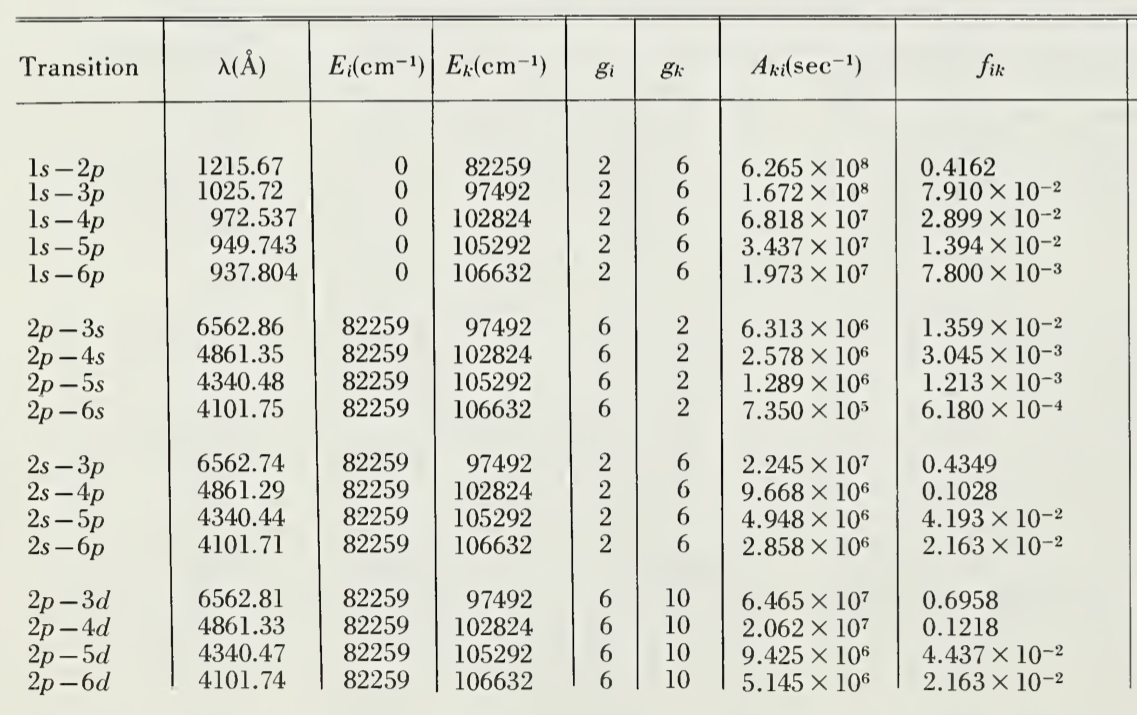
\includegraphics[scale=0.3]{h-alpha-line.png}
\end{center}

\noindent
The $3\rightarrow2$ transitions emit the bright red H-$\alpha$ line.

\begin{center}
\begin{tabular}{|c|c|c|}
\hline
Transition & $\lambda$ (\AA) & $A_{ki}$ ($\text{second}^{-1}$)
\\
\hline
$2p-3s$ & 6562.86 & $6.313\times10^6$
\\
$2s-3p$ & 6562.74 & $2.245\times10^7$
\\
$2p-3d$ & 6562.81 & $6.465\times10^7$
\\
\hline
\end{tabular}
\end{center}

\noindent
Let us compute the spontaneous emission coefficients $A_{ki}$
for H-$\alpha$ and see if the results match the table.

\bigskip
\noindent
The orbital names correspond to the following angular momenta.

\begin{center}
\begin{tabular}{|c|c|}
\hline
Letter & Angular momentum $\ell$
\\
\hline
$s$ & $0$
\\
$p$ & $1$
\\
$d$ & $2$
\\
\hline
\end{tabular}
\end{center}

\noindent
Because of the magnetic quantum number $m_\ell$ there are multiple processes for each transition.

\bigskip
\noindent
There are three processes for the transition $3s\rightarrow2p$.
\begin{align*}
\psi_{3,0,0}&\rightarrow\psi_{2,1,0}
\\
\psi_{3,0,0}&\rightarrow\psi_{2,1,0}
\\
\psi_{3,0,0}&\rightarrow\psi_{2,1,-1}
\end{align*}

\noindent
There are three processes for the transition $3p\rightarrow2s$.
\begin{align*}
\psi_{3,1,1}&\rightarrow\psi_{2,0,0}
\\
\psi_{3,1,0}&\rightarrow\psi_{2,0,0}
\\
\psi_{3,1,-1}&\rightarrow\psi_{2,0,0}
\end{align*}

\noindent
Finally, there are fifteen processes for the transition $3d\rightarrow2p$.
\begin{align*}
\psi_{3,2,2}&\rightarrow\psi_{2,1,1} &
\psi_{3,2,2}&\rightarrow\psi_{2,1,0} &
\psi_{3,2,2}&\rightarrow\psi_{2,1,-1}
\\
\psi_{3,2,1}&\rightarrow\psi_{2,1,1} &
\psi_{3,2,1}&\rightarrow\psi_{2,1,0} &
\psi_{3,2,1}&\rightarrow\psi_{2,1,-1}
\\
\psi_{3,2,0}&\rightarrow\psi_{2,1,1} &
\psi_{3,2,0}&\rightarrow\psi_{2,1,0} &
\psi_{3,2,0}&\rightarrow\psi_{2,1,-1}
\\
\psi_{3,2,-1}&\rightarrow\psi_{2,1,1} &
\psi_{3,2,-1}&\rightarrow\psi_{2,1,0} &
\psi_{3,2,-1}&\rightarrow\psi_{2,1,-1}
\\
\psi_{3,2,-2}&\rightarrow\psi_{2,1,1} &
\psi_{3,2,-2}&\rightarrow\psi_{2,1,0} &
\psi_{3,2,-2}&\rightarrow\psi_{2,1,-1}
\end{align*}

\noindent
For each process, $A_{ki}$ can be computed using the following Heisenberg formula.
\begin{equation*}
A_{ki}=\frac{e^2}{3\pi\varepsilon_0\hbar c^3}\,\omega_{ki}^3\,|r_{ki}|^2
\end{equation*}

\noindent
The transition frequency $\omega_{ki}$ is given by Bohr's frequency condition.
\begin{equation*}
\omega_{ki}=\frac{1}{\hbar}(E_k-E_i)
\end{equation*}

\noindent
The transition probability (multiplied by a physical constant) is
\begin{equation*}
|r_{ki}|^2
=|x_{ki}|^2
+|y_{ki}|^2
+|z_{ki}|^2
\end{equation*}
For wave functions $\psi$ in spherical coordinates we have the following transition amplitudes.
\begin{align*}
x_{ki}&=\int\psi_k^*\,(r\sin\theta\cos\phi)\,\psi_i\,dV
\\
y_{ki}&=\int\psi_k^*\,(r\sin\theta\sin\phi)\,\psi_i\,dV
\\
z_{ki}&=\int\psi_k^*\,(r\cos\theta)\,\psi_i\,dV
\end{align*}

\noindent
The average $A_{ki}$ is obtained by summing over $m_\ell$ states
and dividing by the number of distinct initial states.

\bigskip
\noindent
Using Eigenmath we obtain
\begin{align*}
A_{3s2p}&=6.31358\times10^6\,\text{second}^{-1}
\\
A_{3p2s}&=2.24483\times10^7\,\text{second}^{-1}
\\
A_{3d2p}&=6.4651\times10^7\,\text{second}^{-1}
\end{align*}
which is very close to the values shown in the table.

\end{document}
